\chapter{Interfaces, tensoativos e coloides}\label{ch:b3:colloids}

A maionese é óleo disperso em gotículas de alguns micrômetros em um pouco de
água e vinagre, mantidas separadas pela lecitina e pelas proteínas da gema de
ovo. Batida depressa demais no início, ou com o óleo despejado rápido demais,
ela desanda em uma camada oleosa e outra aquosa: as gotículas se fundem, e a
energia que as mantinha separadas desaparece. O leite, a neblina, a tinta de
escrever, a tinta de parede, o sangue e a água barrenta de um rio são o mesmo
tipo de matéria: partículas ou gotículas muito maiores que as moléculas e muito
menores que qualquer coisa que o olho veja, tão numerosas que a maior parte de
suas moléculas está perto de uma interface. Este capítulo trata da energia das
interfaces, das moléculas que a reduzem, dos \omterm{def:b3:colloids:colloid}{coloides} que as interfaces tornam
possíveis e do que mantém os \omterm{def:b3:colloids:colloid}{coloides} dispersos ou os faz coagular.

\begin{recall}
O volume do 1.º ano chamou de anfifílica uma molécula com uma cabeça hidrofílica e
uma cauda hidrofóbica, e descreveu as interações de London e a permissividade
relativa dos solventes; a parte do 11.º ano do volume escolar encontrou as \omterm{def:b3:colloids:micelle}{micelas}
no sabão. O volume do 2.º ano definiu o potencial químico, a força iônica e a
atividade. O \cref{ch:b3:surfaces-catalysis} tratou da \omterm{def:b3:surfaces-catalysis:adsorption}{adsorção} sobre sólidos, e o
\cref{ch:b3:electrode-kinetics}, da \omterm{def:b3:electrode-kinetics:double-layer}{dupla camada elétrica} e de seu \omterm{def:b3:electrode-kinetics:double-layer}{comprimento de
Debye}. Da física: o movimento browniano e a pressão no interior de uma superfície
curva.
\end{recall}

\begin{omfigure}
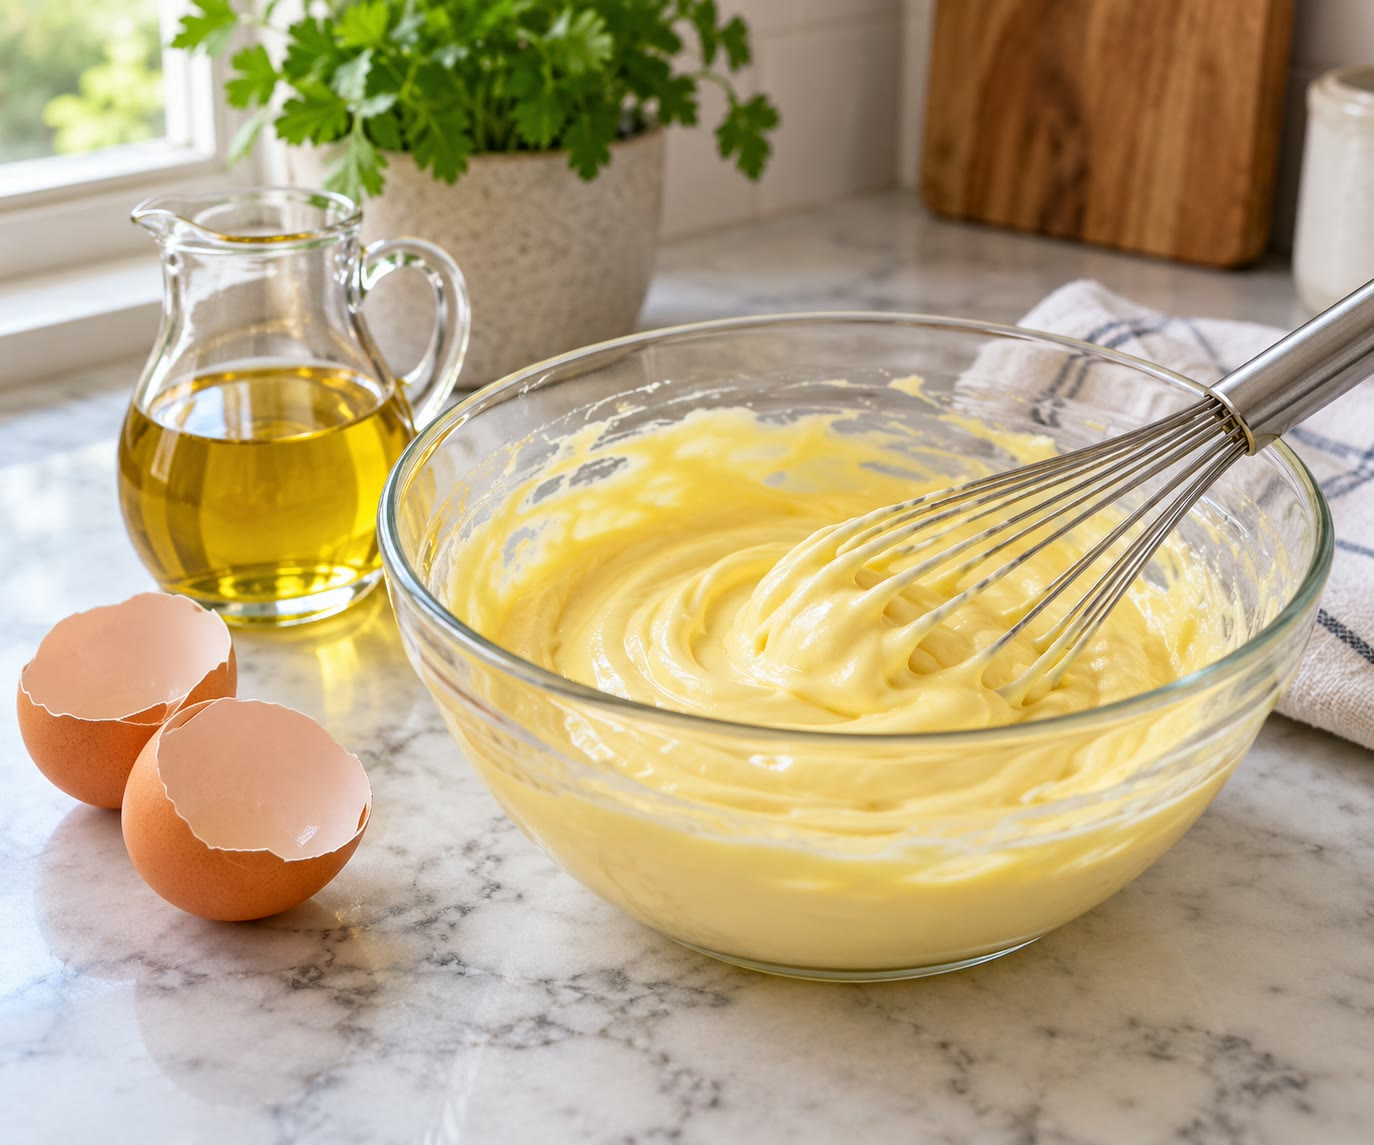
\includegraphics[width=0.6\linewidth]{images/book4/ai/b3-17-mayonnaise.jpg}

{\small Maionese sendo batida: uma \omterm{def:b3:colloids:colloid}{emulsão} de gotículas de óleo em água,
estabilizada pelos \omterm{def:b3:colloids:surfactant}{tensoativos} da gema de ovo.}
\end{omfigure}

\section{Interfaces e tensão superficial}

Uma molécula no seio de um líquido é atraída igualmente em todas as direções; na
superfície, ela perde parte de seus vizinhos. Criar superfície custa energia.

\begin{definition}[Tensão superficial]\label{def:b3:colloids:surface-tension}
A \emph{tensão superficial}\index{tensao superficial@tensão superficial} $\gamma$ de um líquido é a energia de
Gibbs necessária para criar uma unidade de área de sua superfície a temperatura,
pressão e composição constantes: $\gamma = (\partial G/\partial A)_{T,p,n}$, em \unit{J.m^{-2}} $=$ \unit{N.m^{-1}}. Para
uma interface entre duas fases, é a tensão interfacial.
\end{definition}

A água, mantida coesa por ligações de hidrogênio, tem uma \omterm{def:b3:colloids:surface-tension}{tensão superficial} alta:
\qty{72.0}{mN/m} a \qty{25}{\celsius}. Os alcanos têm cerca de 20; o mercúrio, cerca de 480.

\begin{proposition}[Pressão de Laplace]\label{prop:b3:colloids:laplace}
A pressão no interior de uma gota ou de uma bolha esférica de raio $r$ excede a
pressão exterior de
\[
  \Delta p = \frac{2\gamma}{r} .
\]
\end{proposition}

\begin{proof}
Aumente o raio de $\dd r$ no equilíbrio: o trabalho realizado pela diferença de
pressão, $\Delta p\,4\pi r^2\dd r$, é igual ao aumento da energia de Gibbs de superfície, $\gamma\,8\pi r\,\dd r$.
\end{proof}

\begin{definition}[Ângulo de contato, molhamento]\label{def:b3:colloids:wetting}
O \emph{ângulo de contato}\index{angulo de contato@ângulo de contato} $\theta$ de uma gota sobre um
sólido é o ângulo, medido através do líquido, entre a superfície do sólido e a
superfície do líquido na linha onde se encontram sólido, líquido e vapor. Um
líquido \emph{molha}\index{molhamento} o sólido quando $\theta < 90^\circ$, e se espalha
completamente quando $\theta = 0$.
\end{definition}

\begin{theorem}[Equação de Young]\label{thm:b3:colloids:young}
No equilíbrio, as três tensões interfaciais e o \omterm{def:b3:colloids:wetting}{ângulo de contato} satisfazem
\[
  \gamma_{\mathrm{SV}} = \gamma_{\mathrm{SL}} + \gamma_{\mathrm{LV}}\cos\theta .
\]
Esta é a \emph{equação de Young}\index{equacao de Young@equação de Young}.
\end{theorem}

\begin{proof}
Desloque a linha de contato para fora de $\dd x$ (por unidade de comprimento da linha):
uma área $\dd x$ de interface sólido--vapor é substituída por interface sólido--líquido,
e a interface líquido--vapor cresce de $\dd x\cos\theta$. A energia de Gibbs varia de
$(\gamma_{\mathrm{SL}} - \gamma_{\mathrm{SV}} + \gamma_{\mathrm{LV}}\cos\theta)\dd x$, que é nulo no equilíbrio.
\end{proof}

\begin{omfigure}
\begin{tikzpicture}[font=\small, >=Stealth]
  \fill[black!12] (-3.6,-0.5) rectangle (3.6,0);
  \draw[thick] (-3.6,0) -- (3.6,0);
  \node[anchor=north] at (2.6,-0.05) {sólido};
  \fill[omWater!60] (-2.0,0) arc[start angle=160, end angle=20, radius=2.13] -- cycle;
  \draw[thick, omDef] (-2.0,0) arc[start angle=160, end angle=20, radius=2.13];
  % circle centre 0.73 below the solid: a cap smaller than a hemisphere, contact angle 90 - 20 = 70 deg;
  % at the right contact point the liquid surface leaves at 110 deg (up and to the left)
  \draw[->, thick, omThm] (2.0,0) -- ++(110:1.3) node[anchor=south] {$\gamma_{\mathrm{LV}}$};
  \draw[->, thick] (2.0,0) -- (3.3,0) node[anchor=south] {$\gamma_{\mathrm{SV}}$};
  \draw[->, thick] (2.0,0) -- (0.7,0) node[anchor=north, yshift=-1pt] {$\gamma_{\mathrm{SL}}$};
  \draw (1.45,0) arc[start angle=180, end angle=110, radius=0.55];
  \node at (1.33,0.42) {$\theta$};
  \node at (0,0.6) {líquido};
  \node at (-2.8,1.4) {vapor};
\end{tikzpicture}

{\small Uma gota séssil e as três tensões que puxam sua linha de contato: o
equilíbrio de suas componentes ao longo do sólido dá a \omterm{thm:b3:colloids:young}{equação de Young}; aqui $\theta
\approx 70^\circ$, um líquido que \omterm{def:b3:colloids:wetting}{molha} parcialmente.}
\end{omfigure}

\begin{theorem}[Equação de Kelvin]\label{thm:b3:colloids:kelvin}
A pressão de vapor de uma gota esférica de raio $r$ excede a do líquido plano,
$p^*$:
\[
  \ln\frac{p}{p^*} = \frac{2\gamma V_{\mathrm m}}{rRT},
\]
com $V_{\mathrm m}$ o volume molar do líquido. Esta é a \emph{equação de
Kelvin}\index{equacao de Kelvin@equação de Kelvin}.
\end{theorem}

\begin{proof}
O líquido da gota está sob a pressão extra $2\gamma/r$, que eleva seu potencial
químico de $V_{\mathrm m}\,2\gamma/r$ (com $(\partial\mu/\partial p)_T = V_{\mathrm m}$, o líquido sendo incompressível).
O vapor em equilíbrio com ele deve ter seu potencial químico elevado da mesma
quantidade: $RT\ln(p/p^*) = 2\gamma V_{\mathrm m}/r$.
\end{proof}

Para uma gotícula de água de raio \qty{10}{nm} a \qty{25}{\celsius}, $2\gamma V_{\mathrm m}/rRT = 0.105$: sua pressão
de vapor fica 11\,\% acima da da água plana. As gotículas pequenas evaporam enquanto
as grandes crescem, e as nuvens precisam de núcleos para começar; o mesmo vale para
a solubilidade dos cristais pequenos.

\begin{definition}[Amadurecimento de Ostwald]\label{def:b3:colloids:ripening}
O \emph{amadurecimento de Ostwald}\index{amadurecimento de Ostwald} é o crescimento das
partículas ou gotículas maiores de uma dispersão à custa das menores,
impulsionado pela solubilidade ou pela pressão de vapor mais altas das partículas pequenas.
\end{definition}

\section{Tensoativos e micelas}

\begin{definition}[Tensoativo]\label{def:b3:colloids:surfactant}
Um \emph{tensoativo}\index{tensoativo} (agente de superfície) é uma molécula anfifílica
que se adsorve nas interfaces e reduz sua tensão. É um \emph{tensoativo
aniônico}\index{tensoativo anionico@tensoativo aniônico} se sua cabeça é um ânion (dodecilsulfato de
sódio, sabões), um \emph{tensoativo catiônico}\index{tensoativo cationico@tensoativo catiônico}
se é um cátion (sais de amônio quaternário), um \emph{tensoativo não
iônico}\index{tensoativo nao ionico@tensoativo não iônico} se a cabeça é um grupo polar neutro (uma
cadeia de unidades de óxido de etileno).
\end{definition}

\begin{definition}[Concentração de excesso superficial]\label{def:b3:colloids:surface-excess}
A \emph{concentração de excesso superficial}\index{concentracao de excesso superficial@concentração de excesso superficial} $\Gamma$ de um
soluto é a quantidade de soluto na interface por unidade de área, em excesso em
relação à que o mesmo volume conteria se a concentração do seio da solução se
mantivesse até a interface.
\end{definition}

\begin{theorem}[Isoterma de adsorção de Gibbs]\label{thm:b3:colloids:gibbs-adsorption}
Para uma solução diluída de um soluto não iônico de concentração $c$,
\[
  \Gamma = -\frac{1}{RT}\frac{\dd\gamma}{\dd\ln c};
\]
para um \omterm{def:b3:colloids:surfactant}{tensoativo} iônico 1:1 sem sal adicionado, $RT$ é substituído por $2RT$. Esta
é a \emph{isoterma de adsorção de Gibbs}\index{isoterma de adsorcao de Gibbs@isoterma de adsorção de Gibbs}.
\end{theorem}

\begin{proof}
Para a interface, o análogo da relação de Gibbs--Duhem a $T$ e $p$ constantes é
$\dd\gamma = -\sum_i\Gamma_i\,\dd\mu_i$ (a energia de Gibbs de superfície $\gamma A$ faz o papel de $G$,
admitido). Escolhendo a superfície divisória de modo que o solvente não tenha
excesso, $\dd\gamma = -\Gamma\,\dd\mu$, e em uma solução diluída $\dd\mu = RT\,\dd\ln c$. Para um \omterm{def:b3:colloids:surfactant}{tensoativo}
iônico, o cátion e o ânion são ambos adsorvidos com o mesmo excesso, e $\dd\mu$ se torna
$2RT\,\dd\ln c$.
\end{proof}

Um \omterm{def:b3:colloids:surfactant}{tensoativo} cuja \omterm{def:b3:colloids:surface-tension}{tensão superficial} cai linearmente com $\ln c$ tem um excesso
superficial constante: a interface está saturada, e $1/(\Gamma N_A)$ é a área ocupada
por uma molécula adsorvida.

\begin{method}[Área por molécula a partir de uma inclinação $\gamma$--$\ln c$]\label{met:b3:colloids:surface-excess}
\begin{enumerate}
  \item Meça $\gamma$ em função de $c$ abaixo da CMC; trace $\gamma$ em função de $\ln c$.
  \item Tome a inclinação da parte linear logo abaixo da CMC; $\Gamma = -\text{inclinação}/(nRT)$, $n
        = 1$ para um \omterm{def:b3:colloids:surfactant}{tensoativo não iônico}, 2 para um iônico 1:1 sem sal.
  \item Área por molécula $= 1/(\Gamma N_A)$; os valores típicos vão de 0.3 a \qty{0.6}{nm^2}.
\end{enumerate}
\end{method}

\begin{definition}[Micela, concentração micelar crítica, número de agregação]\label{def:b3:colloids:micelle}
Uma \emph{micela}\index{micela} é um agregado de moléculas de \omterm{def:b3:colloids:surfactant}{tensoativo} em solução
cujas caudas hidrofóbicas formam um núcleo de tipo líquido protegido da água
pelas cabeças. A \emph{concentração micelar crítica}\index{concentracao micelar critica@concentração micelar crítica}
(CMC) é a concentração acima da qual se formam micelas; seu número médio de
moléculas é o \emph{número de agregação}\index{numero de agregacao@número de agregação}.
\end{definition}

\begin{proposition}[Rupturas na CMC]\label{prop:b3:colloids:cmc-break}
Acima da CMC, a concentração de \omterm{def:b3:colloids:surfactant}{tensoativo} livre, e com ela a \omterm{def:b3:colloids:surface-tension}{tensão superficial} e
a pressão osmótica, permanecem quase constantes; as propriedades que dependem das
moléculas livres mudam de inclinação na CMC.
\end{proposition}

\begin{proof}[Demonstração parcial]
Trate as \omterm{def:b3:colloids:micelle}{micelas} como uma fase separada: o \omterm{def:b3:colloids:surfactant}{tensoativo} adicionado passa às \omterm{def:b3:colloids:micelle}{micelas}
assim que o potencial químico das moléculas livres atinge o de uma molécula em uma
\omterm{def:b3:colloids:micelle}{micela}, e esse potencial químico, logo a concentração livre, permanece então fixo.
A \omterm{def:b3:colloids:surface-tension}{tensão superficial}, fixada pelas moléculas livres por meio da isoterma de Gibbs,
para de cair; a condutividade continua a subir, mas mais devagar, já que as \omterm{def:b3:colloids:micelle}{micelas}
carregam menos carga por \omterm{def:b3:colloids:surfactant}{tensoativo} que os íons livres (parte de seus contraíons está
ligada). O modelo é um limite, pois as \omterm{def:b3:colloids:micelle}{micelas} de tamanho finito se formam em uma
faixa estreita de concentração (admitido).
\end{proof}

\begin{method}[A CMC a partir de uma ruptura]\label{met:b3:colloids:cmc}
\begin{enumerate}
  \item Meça a \omterm{def:b3:colloids:surface-tension}{tensão superficial} (ou, para um \omterm{def:b3:colloids:surfactant}{tensoativo} iônico, a condutividade)
        em uma faixa de concentrações que abranja a CMC esperada.
  \item Ajuste retas aos dois ramos ($\gamma$ em função de $\log c$, ou $\kappa$ em função de $c$).
  \item Sua interseção é a CMC.
\end{enumerate}
\end{method}

\begin{omfigure}
\begin{tikzpicture}
\begin{axis}[name=gm, width=0.47\linewidth, height=5.2cm, xmin=-5, xmax=-1.5, ymin=30, ymax=76,
  axis lines=left, xlabel={$\log(c/\unit{mol.L^{-1}})$}, ylabel={$\gamma$ / \unit{mN.m^{-1}}},
  tick label style={font=\small}, label style={font=\small}]
\addplot[omDef, very thick] table[x=logc, y=gamma_mN] {figdata/out/bachelor-3-surfactant-cmc-gamma.dat};
\draw[black!40, dashed] (axis cs:-2.086,30) -- (axis cs:-2.086,70);
\node[font=\scriptsize, anchor=south west] at (axis cs:-2.05,45) {CMC};
\end{axis}
\begin{axis}[at={(gm.east)}, anchor=west, xshift=1.4cm, width=0.47\linewidth, height=5.2cm,
  xmin=0, xmax=20, ymin=0, ymax=1.0, axis lines=left, xlabel={$c$ / mM},
  ylabel={$\kappa$ / \unit{mS.cm^{-1}}}, tick label style={font=\small}, label style={font=\small}]
\addplot[omThm, very thick] table[x=c_mM, y=kappa] {figdata/out/bachelor-3-surfactant-cmc-kappa.dat};
\draw[black!40, dashed] (axis cs:8.2,0) -- (axis cs:8.2,0.9);
\node[font=\scriptsize, anchor=south west] at (axis cs:8.4,0.15) {CMC};
\end{axis}
\end{tikzpicture}

{\small Um \omterm{def:b3:colloids:surfactant}{tensoativo} iônico-modelo com a CMC do dodecilsulfato de sódio,
\qty{8.2}{mM} a \qty{25}{\celsius}. À esquerda: a \omterm{def:b3:colloids:surface-tension}{tensão superficial} cai com $\log c$, linearmente logo
abaixo da CMC (uma interface saturada, com cerca de \qty{0.6}{nm^2} por molécula), e
depois permanece constante. À direita: a condutividade sobe menos depressa acima da CMC.}
\end{omfigure}

\begin{definition}[Parâmetro de empacotamento]\label{def:b3:colloids:packing}
O \emph{parâmetro de empacotamento}\index{parametro de empacotamento@parâmetro de empacotamento} de um \omterm{def:b3:colloids:surfactant}{tensoativo} é $P =
v/(a_0l)$, onde $v$ é o volume de sua cauda hidrofóbica, $l$ o comprimento da cauda
estendida e $a_0$ a área ótima por grupo de cabeça na superfície do agregado.
\end{definition}

\begin{proposition}[Forma dos agregados]\label{prop:b3:colloids:packing}
As \omterm{def:b3:colloids:micelle}{micelas} esféricas exigem $P \le \frac13$, as \omterm{def:b3:colloids:micelle}{micelas} cilíndricas $\frac13 < P \le \frac12$, as bicamadas
planas (vesículas, membranas) $\frac12 < P \le 1$; $P > 1$ dá estruturas invertidas.
\end{proposition}

\begin{proof}
Em uma esfera de raio $R \le l$ formada por $N$ moléculas, $Nv = \frac43\pi R^3$ e $Na_0 = 4\pi R^2$, logo
$v/a_0 = R/3 \le l/3$: $P \le \frac13$. Para um cilindro de raio $R$ e comprimento $L$, $Nv = \pi R^2L$ e
$Na_0 = 2\pi RL$: $v/a_0 = R/2 \le l/2$. Para uma bicamada de espessura $2l$ e área $A$, $Nv = 2lA$ e
$Na_0 = 2A$: $v/a_0 = l$.
\end{proof}

\begin{omfigure}
\begin{tikzpicture}[font=\scriptsize]
  % a sphere-forming cone
  \draw[omDef, thick, fill=omDef!15] (0,0) -- (-0.45,1.2) arc[start angle=180, end angle=0, radius=0.45] -- cycle;
  \node at (0,-0.3) {$P < \frac13$: cone};
  % micelle
  \begin{scope}[xshift=2.2cm, yshift=0.6cm]
    \foreach \a in {0,30,...,330}{\draw[black!60] (\a:0.2) -- (\a:0.62); \fill[omDef] (\a:0.7) circle (0.09);}
    \node at (0,-1.05) {micela esférica};
  \end{scope}
  % truncated cone
  \begin{scope}[xshift=4.7cm]
    \draw[omDef, thick, fill=omDef!15] (-0.18,0) -- (-0.4,1.2) -- (0.4,1.2) -- (0.18,0) -- cycle;
    \node at (0,-0.3) {$\frac13 < P < \frac12$};
  \end{scope}
  \begin{scope}[xshift=6.9cm, yshift=0.6cm]
    \fill[omDef!10] (-0.9,-0.55) rectangle (0.9,0.55);
    \foreach \x in {-0.8,-0.5,...,0.8}{\fill[omDef] (\x,0.62) circle (0.08); \fill[omDef] (\x,-0.62) circle (0.08);}
    \node at (0,-1.05) {cilindro (de lado)};
  \end{scope}
  % cylinder shape
  \begin{scope}[xshift=9.4cm]
    \draw[omDef, thick, fill=omDef!15] (-0.3,0) rectangle (0.3,1.2);
    \node at (0,-0.3) {$P \approx 1$: cilindro};
  \end{scope}
  \begin{scope}[xshift=11.4cm, yshift=0.6cm]
    \foreach \x in {-0.8,-0.6,...,0.8}{
      \draw[black!60] (\x,0.5) -- (\x,0.05) (\x,-0.5) -- (\x,-0.05);
      \fill[omDef] (\x,0.58) circle (0.08); \fill[omDef] (\x,-0.58) circle (0.08);}
    \node at (0,-1.05) {bicamada};
  \end{scope}
\end{tikzpicture}

{\small Forma molecular e forma do agregado. Um \omterm{def:b3:colloids:surfactant}{tensoativo} de cabeça grande e cauda
única (um cone) se empacota em \omterm{def:b3:colloids:micelle}{micelas} esféricas; com uma cabeça menor, em cilindros;
uma molécula tão larga na cauda quanto na cabeça, como um lipídio de duas cadeias, em
bicamadas planas, as paredes das vesículas e das membranas celulares.}
\end{omfigure}

A detergência combina esses efeitos: o \omterm{def:b3:colloids:surfactant}{tensoativo} reduz a tensão interfacial entre a
água e uma sujeira oleosa até que a sujeira se enrole em gotas, que as \omterm{def:b3:colloids:micelle}{micelas} então
solubilizam em seus núcleos.

\section{Coloides}

\begin{definition}[Coloide]\label{def:b3:colloids:colloid}
Um \emph{coloide}\index{coloide} é uma dispersão de partículas, gotículas ou bolhas,
de aproximadamente \qty{1}{nm} a \qty{1}{\micro m} (a \emph{fase dispersa}\index{fase dispersa}),
em um \emph{meio dispersante}\index{meio dispersante} contínuo. Um
\emph{sol}\index{sol} é uma dispersão de partículas sólidas em um líquido; uma
\emph{emulsão}\index{emulsao@emulsão}, de gotículas de um líquido em outro líquido; uma
\emph{espuma}\index{espuma}, de bolhas de gás em um líquido ou em um sólido; um \emph{gel}\index{gel},
uma rede de partículas ou de polímeros que se estende por todo o líquido e o torna
semelhante a um sólido; um \emph{aerossol}\index{aerossol}, de gotículas ou partículas em um gás.
\end{definition}

As partículas coloidais são pequenas o bastante para permanecer em suspensão graças
ao movimento browniano (os choques aleatórios das moléculas do solvente, da física) e
grandes o bastante para espalhar a luz.

\begin{definition}[Efeito Tyndall]\label{def:b3:colloids:tyndall}
O \emph{efeito Tyndall}\index{efeito Tyndall} é o espalhamento da luz pelas partículas
de um \omterm{def:b3:colloids:colloid}{coloide}, que torna um feixe visível de lado quando ele atravessa o \omterm{def:b3:colloids:colloid}{coloide},
enquanto uma solução verdadeira permanece invisível.
\end{definition}

\begin{omfigure}
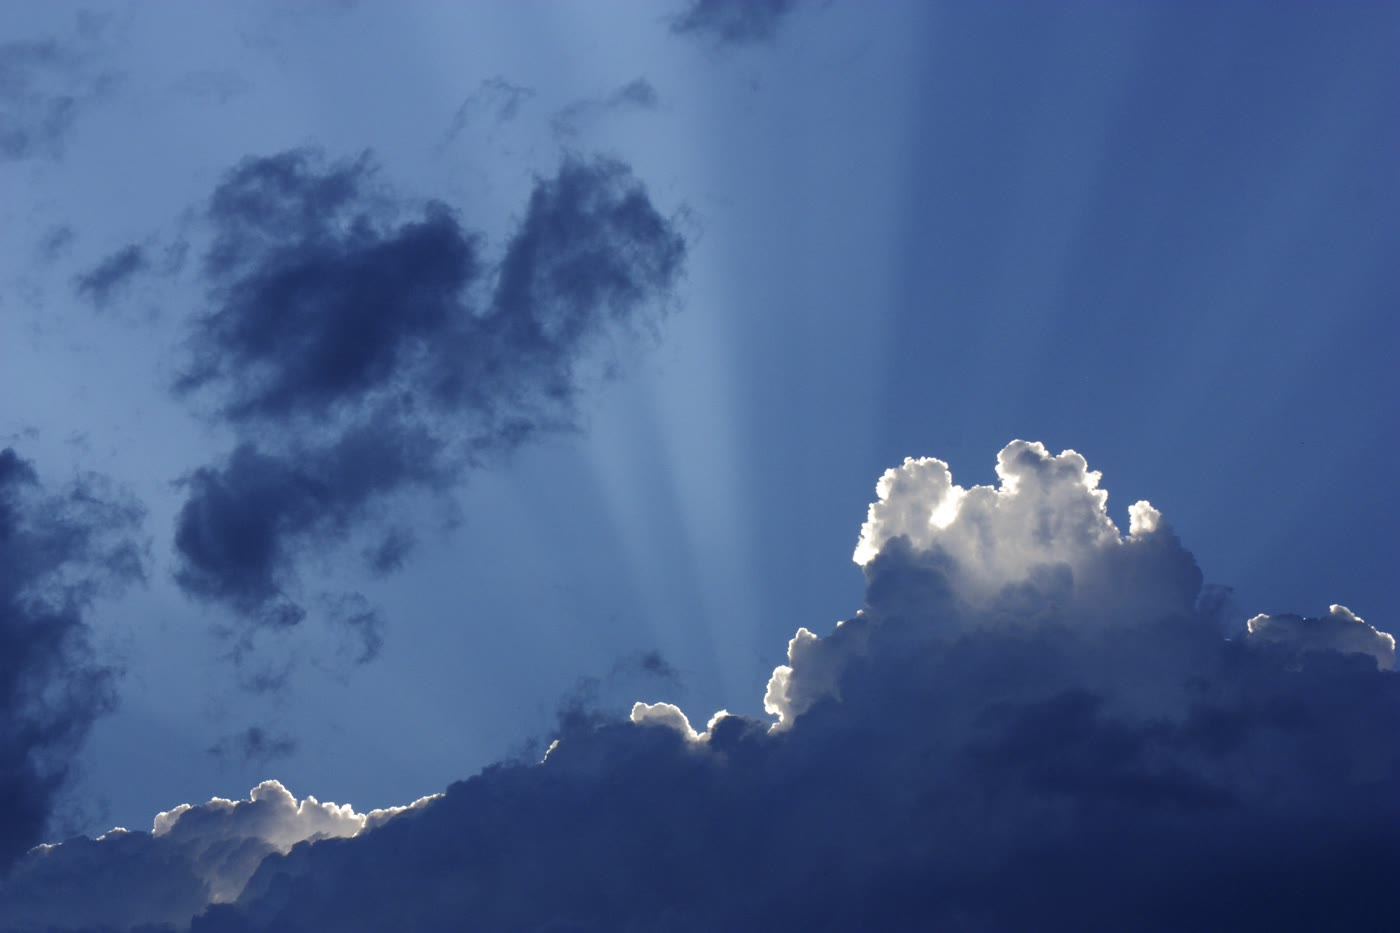
\includegraphics[width=0.55\linewidth]{images/book4/tyndall-sky.jpg}

{\small Raios de sol atravessando uma abertura nas nuvens: eles são visíveis porque o
\omterm{def:b3:colloids:colloid}{aerossol} do ar, gotículas e poeira, espalha parte da luz para os lados, o \omterm{def:b3:colloids:tyndall}{efeito
Tyndall} na escala do céu.}
\end{omfigure}

\section{Estabilidade coloidal}

Duas partículas coloidais sempre se atraem a curta distância pelas forças de van der
Waals. Na água, a maioria das partículas também carrega uma carga (grupos de superfície
ionizados, íons adsorvidos), cercada por uma \omterm{def:b3:electrode-kinetics:double-layer}{camada difusa} de contraíons, a dupla
camada do \cref{ch:b3:electrode-kinetics}. Quando duas partículas se aproximam, suas
\omterm{def:b3:electrode-kinetics:double-layer}{camadas difusas} se sobrepõem e se repelem.

\begin{definition}[Potencial zeta]\label{def:b3:colloids:zeta}
O \emph{potencial zeta}\index{potencial zeta} $\zeta$ de uma partícula é o potencial
elétrico em seu plano de cisalhamento, a fronteira, dentro da dupla camada, entre o
líquido que se move com a partícula e o líquido que não se move; ele é medido a partir
da velocidade das partículas em um campo elétrico (eletroforese).
\end{definition}

\begin{omfigure}
\begin{tikzpicture}[font=\scriptsize]
  \fill[black!20] (0,0) circle (1.2);
  \foreach \a in {0,30,...,330}{\node at (\a:1.05) {$-$};}
  \draw[omDef, dashed] (0,0) circle (1.55);
  \foreach \a in {15,45,...,345}{\draw[omDef, fill=omDef!15] (\a:1.38) circle (0.11); \node at (\a:1.38) {\tiny$+$};}
  \draw[omThm, thick, densely dotted] (0,0) circle (1.85);
  \foreach \a/\r/\s in {10/2.2/+, 50/2.5/+, 95/2.3/-, 130/2.7/+, 175/2.2/+, 215/2.6/-, 250/2.3/+, 290/2.8/+, 345/2.6/+}{
    \draw[black!60, fill=white] (\a:\r) circle (0.11); \node at (\a:\r) {\tiny$\s$};}
  \draw[->, black!60] (2.6,1.6) node[anchor=west] {camada de Stern} -- (40:1.6);
  \draw[->, omThm] (2.6,-1.4) node[anchor=west] {plano de cisalhamento: $\zeta$} -- (-30:1.87);
  \node at (0,0) {partícula};
  \node[anchor=west] at (2.9,0.2) {camada difusa};
\end{tikzpicture}

{\small Uma partícula carregada negativamente com sua dupla camada: uma camada compacta
de Stern de contraíons, o plano de cisalhamento logo além dela, onde se define o
\omterm{def:b3:colloids:zeta}{potencial zeta}, e a \omterm{def:b3:electrode-kinetics:double-layer}{camada difusa}, na qual os contraíons superam os coíons em número
sobre alguns \omterm{def:b3:electrode-kinetics:double-layer}{comprimentos de Debye}.}
\end{omfigure}

\begin{theorem}[Teoria DLVO]\label{thm:b3:colloids:dlvo}
Para duas esferas de raio $a$ separadas por uma distância $h \ll a$, com potencial da \omterm{def:b3:electrode-kinetics:double-layer}{camada difusa}
$\psi$ e constante de Hamaker $A$, a energia de interação é, para potenciais baixos,
\[
  V(h) = 2\pi\varepsilon_r\varepsilon_0a\psi^2\ln\bigl(1 + \eu^{-\kappa h}\bigr) - \frac{Aa}{12h} .
\]
O primeiro termo, a repulsão da dupla camada, decai sobre o \omterm{def:b3:electrode-kinetics:double-layer}{comprimento de Debye} $\kappa^{-1}$;
o segundo, a atração de van der Waals, não depende do sal. Sua soma tem uma barreira
de energia a alguns \omterm{def:b3:electrode-kinetics:double-layer}{comprimentos de Debye} quando a concentração de sal é baixa, e
nenhuma acima de uma concentração crítica.
\end{theorem}

\begin{proof}[Demonstração parcial]
As duas formas são admitidas (a repulsão a partir da sobreposição de duas camadas de
Gouy--Chapman na aproximação de Derjaguin, a atração somando as interações de London
sobre os dois corpos). Aumentar a força iônica aumenta $\kappa$
(\cref{prop:b3:electrode-kinetics:debye-length}): a repulsão se extingue então a um
$h$ menor, onde a atração, que cresce como $1/h$, é mais forte; o máximo de $V$
diminui e acaba desaparecendo.
\end{proof}

\begin{omfigure}
\begin{tikzpicture}
\begin{axis}[width=0.72\linewidth, height=5.6cm, xmin=0, xmax=30, ymin=-40, ymax=45,
  axis lines=left, xlabel={distância $h$ / nm}, ylabel={$V/kT$},
  tick label style={font=\small}, label style={font=\small},
  legend style={font=\scriptsize, draw=none, at={(0.98,0.98)}, anchor=north east}, legend cell align=left]
\addplot[omDef, thick] table[x=h_nm, y=I1] {figdata/out/bachelor-3-dlvo.dat};
\addplot[black!60, thick] table[x=h_nm, y=I10] {figdata/out/bachelor-3-dlvo.dat};
\addplot[omThm, thick] table[x=h_nm, y=I50] {figdata/out/bachelor-3-dlvo.dat};
\addplot[black, thick, dashed] table[x=h_nm, y=I200] {figdata/out/bachelor-3-dlvo.dat};
\draw[black!30] (axis cs:0,0) -- (axis cs:30,0);
\legend{\qty{1}{mM}, \qty{10}{mM}, \qty{50}{mM}, \qty{200}{mM}}
\end{axis}
\end{tikzpicture}

{\small Interação DLVO de duas partículas de raio \qty{100}{nm} (modelo: potencial da
\omterm{def:b3:electrode-kinetics:double-layer}{camada difusa} \qty{-30}{mV}, constante de Hamaker \qty{2e-20}{J}) em água com um sal 1:1.
A \qty{1}{mM}, uma barreira de cerca de $40\,kT$ mantém as partículas separadas; a
\qty{10}{mM}, ela cai à metade; perto de \qty{50}{mM}, desaparece, e toda colisão é aderente.}
\end{omfigure}

\begin{definition}[Coagulação e estabilização]\label{def:b3:colloids:stability}
A \emph{coagulação}\index{coagulacao@coagulação} é a agregação de partículas coloidais
causada pela perda de sua repulsão eletrostática; a \emph{floculação}\index{floculacao@floculação}
é a agregação em flocos frouxos, muitas vezes ligados em ponte por polímeros adsorvidos.
A \emph{concentração crítica de coagulação}\index{concentracao critica de coagulacao@concentração crítica de coagulação}
(CCC) de um eletrólito é a concentração acima da qual um \omterm{def:b3:colloids:colloid}{coloide} coagula
rapidamente. A \emph{estabilização estérica}\index{estabilizacao esterica@estabilização estérica}
mantém as partículas separadas com cadeias poliméricas adsorvidas ou enxertadas,
cuja sobreposição custaria entropia.
\end{definition}

\begin{proposition}[Regra de Schulze--Hardy]\label{prop:b3:colloids:schulze-hardy}
Para um \omterm{def:b3:colloids:colloid}{coloide} fortemente carregado, a \omterm{def:b3:colloids:stability}{concentração crítica de coagulação} de um
eletrólito varia como o inverso da sexta potência da carga $z$ de seus contraíons:
$\text{CCC} \propto z^{-6}$, nas razões $1 : \frac{1}{64} : \frac{1}{729}$ para $z = 1, 2, 3$.
\end{proposition}

\begin{proof}[Demonstração parcial]
Trate duas placas planas. A potencial de superfície alto, a repulsão da dupla camada
por unidade de área tende a $V_R = (64nkT/\kappa)\eu^{-\kappa h}$, onde $n$ é a densidade numérica do eletrólito
$z{:}z$, independentemente do potencial (admitido); a atração é $V_A =
-A/(12\pi h^2)$. Na CCC, a barreira acaba de desaparecer: $V = 0$ e $\dd V/\dd h = 0$ na mesma
distância. Como $\dd V_R/\dd h = -\kappa V_R$ e $\dd V_A/\dd h = -2V_A/h$, as duas condições dão
$\kappa V_R = 2V_R/h$, logo $\kappa h = 2$, e então $64nkT\eu^{-2}/\kappa = A\kappa^2/(48\pi)$, isto é, $n \propto \kappa^3$. Com
$\kappa^2 = 2nz^2e^2/(\varepsilon kT)$, $\kappa^3 \propto (nz^2)^{3/2}$ e $n \propto n^{3/2}z^3$: logo $n \propto z^{-6}$.
\end{proof}

\begin{omfigure}
\begin{tikzpicture}[font=\small, >=Stealth]
  \foreach \x/\lab/\v in {0/\ce{Na+}/1, 2.6/\ce{Ca^{2+}}/{1/64}, 5.2/\ce{Al^{3+}}/{1/729}}{
    \node at (\x,0) {\lab};
    \node[font=\scriptsize] at (\x,-0.45) {CCC $\times\,\v$};}
  \draw[->, thick, omDef] (-0.8,-0.95) -- (6.0,-0.95) node[midway, below, font=\scriptsize] {dose menor para coagular um coloide negativo};
\end{tikzpicture}

{\small A regra de Schulze--Hardy para um \omterm{def:b3:colloids:colloid}{coloide} carregado negativamente: a
\omterm{def:b3:colloids:stability}{concentração crítica de coagulação} cai com a sexta potência da carga do contraíon.}
\end{omfigure}

A regra explica por que os sais de alumínio são tão eficazes para clarificar a água,
e por que os rios depositam sua carga de argila onde encontram a água salgada do mar.

\begin{method}[Escolher a dose de coagulante]\label{met:b3:colloids:coagulant-dose}
\begin{enumerate}
  \item Meça a CCC de um eletrólito de referência para a suspensão (ensaios de jarros
        com doses crescentes, observando a sedimentação).
  \item Converta-a para o contraíon do coagulante com a regra de Schulze--Hardy.
  \item Converta em uma massa de sal por metro cúbico com sua fórmula; acrescente o
        suficiente para a hidrólise e para a alcalinidade que ela consome.
  \item Evite a sobredosagem: contraíons muito carregados podem inverter o sinal da
        carga das partículas e reestabilizá-las.
\end{enumerate}
\end{method}

\section{Os coloides em ação}

\begin{definition}[Balanço hidrofílico--lipofílico]\label{def:b3:colloids:hlb}
O \emph{balanço hidrofílico--lipofílico}\index{balanco hidrofilico--lipofilico@balanço hidrofílico--lipofílico}
(HLB) de um \omterm{def:b3:colloids:surfactant}{tensoativo não iônico} é, na escala de Griffin, $20$ vezes a fração mássica
de sua parte hidrofílica: valores baixos (3 a 6) convêm às \omterm{def:b3:colloids:colloid}{emulsões} água em óleo,
valores altos (8 a 18) às \omterm{def:b3:colloids:colloid}{emulsões} óleo em água e aos detergentes.
\end{definition}

As \omterm{def:b3:colloids:colloid}{emulsões} são termodinamicamente instáveis, pois cada gotícula carrega energia
interfacial; os emulsificantes as tornam cineticamente estáveis reduzindo essa
energia e acrescentando em torno de cada gotícula uma camada repulsiva, carregada ou
estérica. A maionese é uma \omterm{def:b3:colloids:colloid}{emulsão} óleo em água com tanto óleo (cerca de quatro
quintos do volume) que as gotículas ficam comprimidas umas contra as outras, o que a
torna um sólido mole. As \omterm{def:b3:colloids:colloid}{espumas} são estabilizadas por \omterm{def:b3:colloids:surfactant}{tensoativos} que retardam a
drenagem dos filmes líquidos entre as bolhas; os antiespumantes, muitas vezes óleos de
silicone, se espalham sobre esses filmes e os rompem. Nas estações de tratamento de
água, os sais de alumínio ou de ferro(III) coagulam a argila e os \omterm{def:b3:colloids:colloid}{coloides} orgânicos
que turvam a água dos rios; o hidróxido que eles formam arrasta os flocos ao
sedimentar. As nanopartículas metálicas são mantidas dispersas por íons citrato
adsorvidos (eletrostática) ou por cadeias poliméricas ligadas por tióis (estérica).

\begin{inthelab}[O anel de du Noüy]
Um anel de platina, flambado para limpá-lo, fica suspenso em uma balança e é imerso
horizontalmente no líquido, depois levantado lentamente. A força necessária para
puxá-lo através da superfície passa por um máximo; dividida pelo dobro da
circunferência do anel e corrigida pela forma do menisco levantado, ela dá a \omterm{def:b3:colloids:surface-tension}{tensão
superficial}. A medida de uma série de \omterm{def:b3:colloids:surfactant}{tensoativos} começa pela solução mais diluída,
enxaguando o anel entre as amostras.
\end{inthelab}

\begin{safety}{\ghs[0.8cm]{GHS02}\ghs[0.8cm]{GHS05}\ghs[0.8cm]{GHS07}}
% ledger: ghs4:SDS, ghs4:Al2SO43
Dodecilsulfato de sódio em pó: sólido inflamável, nocivo se ingerido, provoca lesões
oculares graves, irrita as vias respiratórias; pesado sem levantar poeira, com
proteção ocular. Sulfato de alumínio (\ghs[0.6cm]{GHS05}): provoca lesões oculares
graves.
\end{safety}

\begin{history}[Tyndall e o ultramicroscópio]
John Tyndall mostrou em 1869 que um feixe de luz se torna visível no ar carregado de
partículas finas e invisível no ar livre delas, e que a luz espalhada é azulada e
polarizada. Richard Zsigmondy, que estudava a cor vermelha dos \omterm{def:b3:colloids:colloid}{sóis} de ouro,
construiu com Henry Siedentopf, em 1903, o ultramicroscópio, que ilumina o \omterm{def:b3:colloids:colloid}{coloide} de
lado e mostra cada partícula como um ponto de luz espalhada sobre um fundo escuro,
pequena demais para ser resolvida, mas contável. Ele recebeu o Prêmio Nobel de
Química de 1925 por seus trabalhos sobre os \omterm{def:b3:colloids:colloid}{coloides}.
\end{history}

\section{Exercícios}

\begin{exercise}[$\star$]\label{exo:b3:colloids:1}
% ledger: st:H2O.25C
Calcule a pressão no interior de uma bolha de ar de \qty{1.0}{\micro m} de diâmetro na água
a \qty{25}{\celsius} (exterior: \qty{1.0}{bar}).
\end{exercise}

\begin{exercise}[$\star$]\label{exo:b3:colloids:2}
% ledger: st:H2O.25C
Calcule a pressão de vapor de uma gotícula de água de raio \qty{10}{nm} em relação à da
água plana a \qty{25}{\celsius} ($V_{\mathrm m} = \qty{18.07}{cm^3/mol}$).
\end{exercise}

\begin{exercise}[$\star$]\label{exo:b3:colloids:3}
Um líquido com $\gamma_{\mathrm{LV}} = \qty{72}{mN/m}$ sobre um sólido com $\gamma_{\mathrm{SV}} = \qty{40}{mN/m}$ e $\gamma_{\mathrm{SL}} =
\qty{20}{mN/m}$ (dados do exercício): calcule o \omterm{def:b3:colloids:wetting}{ângulo de contato}. O líquido \omterm{def:b3:colloids:wetting}{molha} o sólido?
\end{exercise}

\begin{exercise}[$\star$]\label{exo:b3:colloids:4}
% ledger: eps:H2O.25C
Calcule o \omterm{def:b3:electrode-kinetics:double-layer}{comprimento de Debye} em água a \qty{25}{\celsius} para \qty{0.010}{mol/L} de NaCl e de
\ce{MgSO4}.
\end{exercise}

\begin{exercise}[$\star\star$]\label{exo:b3:colloids:5}
Logo abaixo de sua CMC, a \omterm{def:b3:colloids:surface-tension}{tensão superficial} de um \omterm{def:b3:colloids:surfactant}{tensoativo} iônico (1:1, sem sal)
cai \qty{12.6}{mN/m} por unidade de $\ln c$ a \qty{25}{\celsius}. Calcule o excesso superficial e
a área por molécula.
\end{exercise}

\begin{exercise}[$\star\star$]\label{exo:b3:colloids:6}
\omterm{def:b3:colloids:surface-tension}{Tensões superficiais} de um \omterm{def:b3:colloids:surfactant}{tensoativo não iônico}: 52.0, 45.5, 39.1, 33.4, 33.3 e
\qty{33.4}{mN/m} em $\log c = -5.0$, $-4.5$, $-4.0$, $-3.5$, $-3.0$ e $-2.5$ (dados do exercício).
Estime a CMC.
\end{exercise}

\begin{exercise}[$\star\star$]\label{exo:b3:colloids:7}
Para o dodecilsulfato de sódio, tome $v = \qty{0.350}{nm^3}$, $l = \qty{1.67}{nm}$ e $a_0 = \qty{0.60}{nm^2}$; para um
lipídio com duas cadeias desse tipo, $2v$, o mesmo $l$ e $a_0 = \qty{0.65}{nm^2}$ (dados do
exercício). Preveja a forma de seus agregados.
\end{exercise}

\begin{exercise}[$\star\star$]\label{exo:b3:colloids:8}
Um \omterm{def:b3:colloids:colloid}{sol} carregado negativamente coagula com \qty{60}{mM} de NaCl. Preveja a CCC com \ce{CaCl2}
e com \ce{AlCl3}. O que faria o \ce{Na3PO4}?
\end{exercise}

\begin{exercise}[$\star\star$]\label{exo:b3:colloids:9}
% ledger: cmc:C12E6
Calcule o HLB de Griffin do éter monododecílico do hexaetilenoglicol,
\ce{C12H25(OCH2CH2)6OH}, cuja parte hidrofílica é $\ce{(OCH2CH2)6OH}$. Ele convém a uma
\omterm{def:b3:colloids:colloid}{emulsão} óleo em água?
\end{exercise}

\begin{exercise}[$\star\star\star$]\label{exo:b3:colloids:10}
Uma dispersão contém gotículas de raio 50 e \qty{500}{nm}. Usando a \omterm{thm:b3:colloids:kelvin}{equação de Kelvin}
aplicada à solubilidade, explique quais crescem e quais encolhem, e por que as
\omterm{def:b3:colloids:colloid}{emulsões} engrossam com o tempo mesmo sem coalescência.
\end{exercise}

\begin{exercise}[$\star\star\star$]\label{exo:b3:colloids:11}
Mostre, a partir da pressão de Laplace, que o líquido sobe até a altura $h = 2\gamma\cos\theta/(\rho gr)$ em um
capilar de raio $r$, e calcule-a para a água ($\theta = 0$, raio de \qty{0.10}{mm}).
\end{exercise}

\begin{exercise}[$\star\star\star$]\label{exo:b3:colloids:12}
Usando a figura DLVO, explique por que a adição de \qty{100}{mM} de NaCl a um \omterm{def:b3:colloids:colloid}{sol} estável
a \qty{1}{mM} o faz coagular, enquanto a adição de um polímero não adsorvido não altera a
barreira, mas um polímero enxertado nas partículas pode mantê-las separadas em qualquer
concentração de sal.
\end{exercise}

% keep the heading with its problem box, which fills a page by itself
\clearpage
\enlargethispage{3\baselineskip}
\section{Problema: Clarificar água barrenta com alúmen}

\begin{problem}[{Problema de fim de semana --- clarificar água barrenta com alúmen:
a dupla camada das partículas de argila, a barreira DLVO, a regra de Schulze--Hardy e
a dose de sulfato de alumínio}]
\label{pb:b3:colloids:1}
% ledger: eps:H2O.25C, visc:H2O.25C
Uma estação de tratamento de água recebe uma água mole e turva: partículas de argila de
raio \qty{100}{nm} e densidade \qty{2650}{kg/m^3}, com potencial da \omterm{def:b3:electrode-kinetics:double-layer}{camada difusa} de \qty{-30}{mV}, em
uma água que contém \qty{1.0}{mM} de \ce{NaHCO3}. Os ensaios de jarros mostram que as partículas
coagulam rapidamente acima de \qty{50}{mM} de NaCl (dados do problema). A estação trata \qty{1000}{m^3}
por hora com sulfato de alumínio, $\ce{Al2(SO4)3}$ ($M = \qty{342.3}{g/mol}$).

\medskip\noindent\textbf{Parte I --- Um \omterm{def:b3:colloids:colloid}{coloide} estável.}
\begin{enumerate}
  \item Por que as partículas de argila na água carregam uma carga negativa?
  \item Calcule a força iônica da água.
  \item Calcule seu \omterm{def:b3:electrode-kinetics:double-layer}{comprimento de Debye}.
  \item Compare-o com o raio das partículas. Que aproximação da fórmula DLVO isso
        justifica?
  \item Calcule a velocidade de sedimentação de uma partícula pela lei de Stokes, $v =
        2\Delta\rho\,gr^2/9\eta$ ($\eta = \qty{0.89}{mPa.s}$), em milímetros por dia.
  \item Por que as partículas não se grudam umas às outras quando colidem?
\end{enumerate}

\medskip\noindent\textbf{Parte II --- A barreira DLVO.}
\begin{enumerate}[resume]
  \item Escreva a energia DLVO de duas partículas.
  \item Leia na figura a barreira a \qty{1}{mM}, em unidades de $kT$.
  \item Com que frequência duas partículas que colidem atravessariam uma barreira assim?
  \item O que acontece com a barreira perto de \qty{50}{mM}?
  \item Explique por que adicionar sal abaixa a barreira.
\end{enumerate}

\medskip\noindent\textbf{Parte III --- Schulze--Hardy.}
\begin{enumerate}[resume]
  \item Enuncie a regra.
  \item Preveja a CCC de \ce{Ca^{2+}}.
  \item Preveja a CCC de \ce{Al^{3+}}.
  \item Por que só os cátions do coagulante importam para esse \omterm{def:b3:colloids:colloid}{coloide}?
  \item Por que o sulfato do alúmen é quase irrelevante para a \omterm{def:b3:colloids:stability}{coagulação}?
\end{enumerate}

\medskip\noindent\textbf{Parte IV --- A dose.}
\begin{enumerate}[resume]
  \item Calcule a quantidade de \ce{Al^{3+}} necessária por metro cúbico.
  \item Deduza a quantidade de $\ce{Al2(SO4)3}$ por metro cúbico.
  \item Deduza sua massa por metro cúbico.
  \item Deduza a massa usada por hora pela estação.
  \item Na água, o \ce{Al^{3+}} se hidrolisa e reage com o hidrogenocarbonato. Escreva a
        equação balanceada que forma \ce{Al(OH)3}.
  \item Que fração do hidrogenocarbonato a dose consome? O pH muda muito?
  \item Por que uma sobredosagem pode tornar a água turva de novo?
  \item Enuncie o resultado: a massa mínima de sulfato de alumínio por metro cúbico.
\end{enumerate}
\end{problem}
